\chapter{Controlling the WebRTC Identity Parameters}
\label{identitynegotiation}
\begin{quote}
\textit{
The WebRTC identity architecture allows to bind the media session to a validated peer identity.
In Chapter~\ref{webrtcprivacy}, we presented privacy issues related to this specification and to \gls{sso} on the Web in general.
From our point of view, the fact that users lack control over which identity services they want to use on the Web is at the heart of these privacy issues.
Furthermore, users may also ask themselves whether they should trust their peers' \gls{idp} and their peers' authentication strength?
In order to raise users' trust in a communication, both from a privacy and a security perspective, we propose to give users more control over WebRTC identity parameters.
Firstly, in Section~\ref{sec_sdp}, we define a \gls{sdp} extension to negotiate the other peer's \gls{idp} and authentication strength during the \gls{sdp} call setup.
We implement our solution which shows that such negotiation mechanism would benefit from more flexibility in the choice of \gls{idp} for peer authentication.
Yet, as we explained previously, \gls{idp} choices are limited on the Web.
The WebRTC identity specification poses some interesting concepts but for the limited scope of user-to-user authentication.
We are interested in studying how it can be extended to support more use cases.
In Section~\ref{webconnect} we present WebConnect, a prototype for an Identity Metasystem \gls{api} based on the WebRTC identity specification.
We show that on the long run, adoption of such an \gls{api} could reduce the implementation burden for websites developers and allow users to preserve their privacy by choosing trusted \gls{idp}.
}
\end{quote}

\begin{figure}[H]
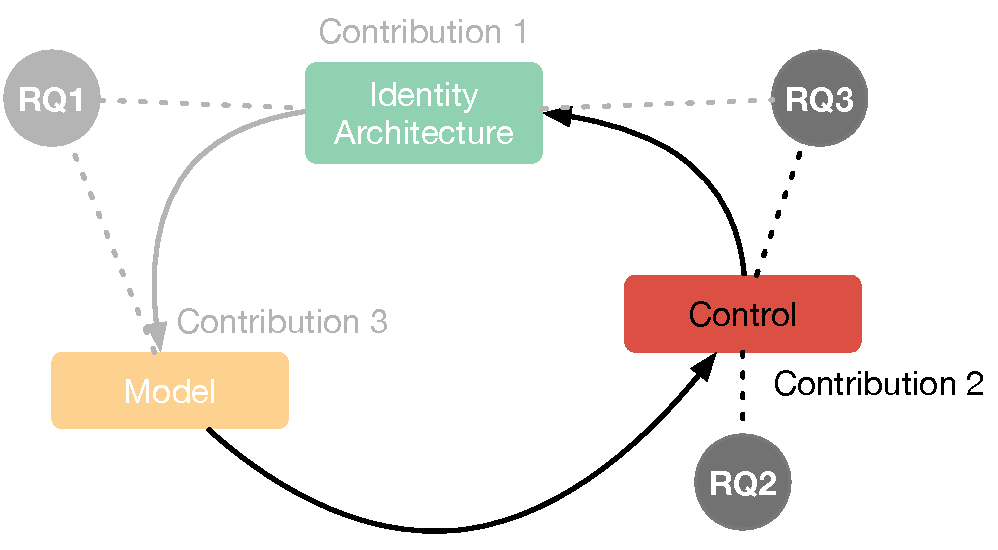
\includegraphics[scale=.5]{images/contrib2}
\caption{Overview of our Contributions: Controlling the WebRTC Identity Parameters.}
\label{contrib2}
\end{figure}

\glsresetall
\section{An SDP Extension to Allow Identity Negotiation}
\label{sec_sdp}

The WebRTC identity specification allows binding the media session to a validated peer identity. 
However, indications as to whether the \gls{idp} and identity assertion should be trusted are limited\footnote{The only guarantee is that the IdP Proxy is loaded over HTTPS.}.
Alice may ask herself the following questions: ``should I trust my peer's \gls{idp}'' and more importantly ``what is the strength of my peer's authentication''?
In order to address RQ2 ``can we act on a WebRTC session to raise the trust and security level'', we propose to let users negotiate their identity parameters.
In this section we thus address the following research question:
\begin{itemize}
\item \textbf{RQ2.1}: How to let users negotiate the other peer's identity parameters?
\end{itemize}

As a peer's authentication strength is known by and depends on the peer's \gls{idp}, trust in the security of the communication depends directly on Alice's trust in her peer's \gls{idp}.
Though Alice may not be capable to evaluate this \gls{idp}'s trustworthiness, she may not have previous relations with this \gls{idp} or, just not enough observable feedback to judge. 
Recommendation from a trusted source could solve Alice's lack of knowledge and allows for identity parameter negotiation. 

\subsection{Recommendation Sources}
Three actors, potentially trusted by the user and already involved in the WebRTC communication setup, would be well-suited to recommend trust in the peer's identity and conduct the identity negotiation. 
These are the user's \gls{cs} and/or its associated client, the user's \gls{idp}, and the browser.
However, each of these actors has a different role and visibility on WebRTC identity management.
We use the following properties to evaluate where to best place the negotiation responsibility:
\begin{itemize}
\item Trusted by the user or not.
\item Capability to recommend trusted \gls{idp}.
\item Knowledge of the call context. 
\end{itemize}

Supposing that Alice is allowed to choose a trusted \gls{idp}, we can consider that Alice's \gls{idp} occupies a trusted position in the communication setup.
As an \gls{idp}, Alice's \gls{idp} would also be well suited to understand and to evaluate other \gls{idp}'s trustworthiness.
However, web \gls{idp} are organised in silos and do not interact with each other.
In order to serve as recommendation sources, they would need to build trusted identity federations, circles of trust, or individual trust relations.
Besides, \gls{idp} are not aware of the call context (used call service, risk level, etc.) and only deal with user authentication. 
Configuring user preferences for call security depending on call context may prove to be difficult. 
%\todo{Vincent :tu es en train de r�inventer les "circle of trust" (CoT) (= une f�d�ration d'\gls{idp} pour servir une communaut� de SP ; chaque \gls{idp} apportant sa sp�cificit� soit pour des attributs, soit pour une m�thode d'authentification, soit encore pour un canal) ; on a bcp travaill� l� dessus il y a qq ann�es ... par exemple le projet FC2. Jean-Michel ne t'en a jamais parl� ? cf. \url{http://competitivite.gouv.fr/projets-en-fin-de-conventionnement-fui/fiche-projet-abouti-576/fc2-187.html?cHash=3de0f6c3a7d3743277baedf0acdcdeea}}

Conversely, the \gls{cs} is fully aware of the call-context and it would be quite simple for users to define separate preferences for each \gls{cs}.
\gls{cs} are also dealing with \gls{idp} to authenticate their own users.
Evaluating the trustworthiness of an authentication from an \gls{idp} they already trust would not be different.
However, \gls{cs} trusting \gls{idp} that they do not implement, \ie without explicit configuration and contractual agreement, would also require a kind of trusted federated identity service.
\gls{cs} may also not be trusted by their user and this is the reason why the WebRTC identity specification exists in the first place.
Even if the user's \gls{cs} is trusted, the WebRTC identity architecture may still be relevant in interoperable scenarios as these involve multiple \gls{cs}.

Finally, the web browser may also be an adequate actor to evaluate the trustworthiness of the other party authentication.
Being the WebRTC Trusted Computing Base, the browser is considered to be trusted. 
It has also some knowledge of the call context, although less than the \gls{cs}, and could easily be configured by the user.
In the current specification, the browser is in charge of \gls{idp}'s origin validation through \gls{https}.
This already constitutes a kind of low-level trust recommendation towards asserting identity assertion security.
However, browsers are not usually dealing with authentication strength and \gls{idp} trustworthiness.
%\todo{Vincent:ici, je pensais que tu aurai cit� TLS-OBS dans ta biblio : \url{https://www.usenix.org/system/files/conference/usenixsecurity12/sec12-final162.pdf} Je ne me souviens plus si on en a parl� ensemble et puis je suis p� hors sujet}

\begin{table}
\begin{tabular}{@{}lccc@{}}\toprule\toprule
  Actors & Trusted & Recommendation & Context\\\midrule
  Identity Provider & + & ++ & - \\
  Communication Service & - & + & ++ \\
  Browser & ++ & - & + \\\bottomrule
  \hline
\end{tabular}
\caption{Comparison of communication setup actors to act as an identity recommendation source. }
\label{tab_comparison}
\end{table}

Table~\ref{tab_comparison} summarises our simple comparison of the \gls{idp}, \gls{cs} and browser as trusted recommendation sources.
None of these three actors appears clearly more suited to evaluate and negotiate over the other party authentication. 
\gls{cs} could implement such functionality as the need arises without waiting for a standardisation process.
However, this raises the question of whether or not the \gls{cs} can be considered as part of the \gls{tcb} for WebRTC call.
Trusted \gls{cs} would probably be more suited for enterprise scenario, but not in the general web ecosystem.
For a more generic identity negotiation implementation working on any WebRTC service, the web browser would be the best suited to implement such functionality.
Indeed, the browser is already responsible for verifying identity assertion but also for the management of \gls{api} and plugin authorizations.
%\todo{This is an important question, but it should also be asked explicitly in the introduction. For now, it's missing.}

\subsection{SDP Extension}
As we described in the previous section, the security of a WebRTC session depends on the peer's authentication strength and the trustworthiness of the \gls{idp} asserting the peer's identity.
Supposing that knowledge of these two parameters is available, a user may act on the session to negotiate a higher security level.
This would either be done by requesting a higher authentication level, or an identity assertion from another \gls{idp}.

To convey these requests in the negotiation we define two identity parameters.
The \gls{acrus}: \texttt{List<ACRValue>}, a list ordered by preference of accepted authentication class values.
And the \gls{orus}: \texttt{List<Origin>}, a list ordered by preference of accepted \gls{idp}'s origins.
The identity assertion is transmitted in \gls{sdp} offer and answer as the \texttt{a=identity} session level attribute (see Section~\ref{sec:webrtcid}).
Defining extensions to this attribute in order to convey identity parameter requests would be possible.
However, the \texttt{identity} attribute grammar specifies that an extension must follow a valid identity assertion.
This implies that it would not be possible to negotiate identity parameters without providing an identity assertion.
However, anonymous calling is often cited as an important use case for communication services~\cite{I-D.copeland-rtcweb-p2p-idp-auth, crom_management_2015}.
The need may arise for a user to negotiate identity parameters while being anonymous.

We instead propose to define a new type of \gls{sdp} session-level attribute to negotiate these identity parameters.
The \gls{acor} \gls{sdp} attribute defines a list of accepted authentication class and \gls{idp} domain for the other peer identity.
\begin{itemize}
\item \texttt{a=acor:LIST<ACRValue> ; List<Origin>}
\end{itemize}

An \gls{sdp} negotiation is a sequence of offer and answer messages, with an offer always followed by an answer. 
We detail two scenarios where the negotiation for identity parameters either starts from an offer or from an answer.
To accept the requested \gls{acor} attributes, a peer must thus reply a \gls{sdp} message with a compatible identity assertion.

%\todo{Vincent :on utilise souvent l'ACR coupl� � l'AMR (par exemple dans le cas de Mobile Connect).
%Est-ce que l'AMR aurait eu un usage dans ton cas (je pense au cas ou deux idp n'offiraient pas les m�mes m�thodes d'authent ce qui pourrait contrarier la mise en relation)}
% -> oui, mais pas eu le temps de r�f�rencer �a avant


\subsubsection{SDP Offer with Identity Request}
Figure~\ref{fig_sdp_offer} shows a sequence diagram of the offer scenario. 
In this scenario, Alice's browser (UA$_A$) gets negotiation parameters from Alice's Recommendation source (R$_A$).
Upon receiving the \gls{sdp} offer and the requested identity parameters, Bob's browser (UA$_B$) checks whether the requested \gls{idp} Origins are acceptable. 
We do not detail the way to get this information or how to select the \gls{idp}, but the solution would probably rely on Bob's Recommendation source (R$_B$) and registered \gls{idp} in UA$_B$.
If no requested origin is available, the browser must answer with a \gls{sdp} containing no identity attribute.
Otherwise, it proceeds to request an assertion from the selected \gls{idp}.
If no requested \gls{acrus} matches the current authentication level a standard \texttt{IdpLoginError} is returned.
If this error does not contain a \texttt{loginURL} parameter, then no requested \gls{acr} are supported by the \gls{idp} and a \gls{sdp} with no identity attribute is returned by UA$_B$.
However, if the error contains a \texttt{loginURL}, the user can be authenticated with a procedure matching one of the \gls{acrus} by following the provided login \gls{url}. 
Once this standard authentication procedure is done, Bob's Assertion (ASSERTION\_B) is returned in the \gls{sdp} answer. 

On receiving ASSERTION\_B, UA$_A$ asks Bob's \gls{idp}, through it's own \gls{idp} Proxy instance, to validate the assertion. 
The \texttt{IdentityValidationResult} returned by the proxy should contain the assertion \gls{acr} value, allowing UA$_A$ to open the media channel. 

\begin{figure*}[tbp]
\begin{center}
    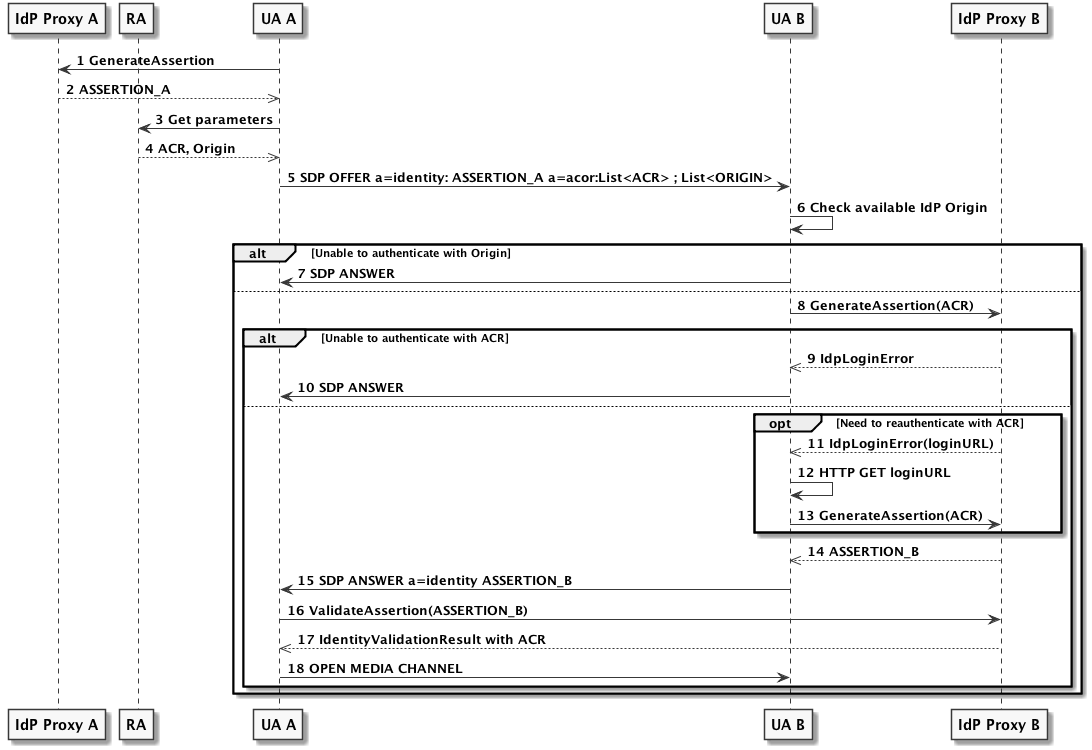
\includegraphics[height=\textwidth, angle =90 ]{images/sdp_offer}
\end{center}
\caption{SDP Offer}
\label{fig_sdp_offer}
\end{figure*}

\subsubsection{SDP Answer with Identity Request}
The answer scenario is similar to the offer scenario but differs in that the assertion is received before the receiving user sent any identity request.
Figure~\ref{fig_sdp_answer} shows a sequence diagram for this scenario.
Upon receiving the offer, UA$_B$ gets identity parameters from R$_B$.
If the received assertion origin is accepted, UA$_B$ checks ASSERTION\_A through a local instance of \gls{idp} Proxy A.
If one of the identity parameters does not match with the received assertion, UA$_B$ returns a \gls{sdp} answer with its identity parameters request.
This would trigger a new offer from UA$_A$ if possible. 

Alternatively, UA$_B$ could accept the first offer and later send a new offer to renegotiate A's identity.

\begin{figure*}[tbp]
\begin{center}
    \includegraphics[height=\textwidth, angle =90 ]{images/sdp_answer}
        %\includegraphics[width=\textwidth]{sdp_answer}
\end{center}
\caption{SDP Answer}
\label{fig_sdp_answer}
\end{figure*}


\subsection{Validation on the current specification}
Both browser and \gls{cs} get access to \gls{sdp} messages during the call setup and could support identity negotiation in a similar way.
The browser would be more difficult to modify than a WebRTC JavaScript client due to its large code base.
In contrast, implementation of identity negotiation at the \gls{idp} level would be something quite different.
As the \gls{idp} does not actually see \gls{sdp} messages, the WebRTC \gls{api} would need to be heavily modified.
This kind of modification to the specification is out of scope of our research\footnote{The definition and evolution of proposed standard is a heavy process. A constraint of our work is to aim for compatibility with existing specification rather than proposing heavy modifications.}.
Our objectives for implementing our solution to negotiate identity parameters over \gls{sdp} are the following:
\begin{itemize}
\item \textbf{}Evaluate the complexity of deploying this solution.
\item Validate the feasibility of an implementation given the current state of WebRTC implementation on web browser.
\item Verify that adding identity parameters does not compromise inter-operability with other services.
\end{itemize}

Ultimately, we implement the negotiation functionalities at the \gls{cs} level and integrate it to our WebRTC service\footnote{Available at \url{https://github.com/Sparika/ACOR\_SDP}}.
Figure~\ref{fig_acorNegotiation} shows the identity request interface.
The web interface allows both users to request new \gls{acrus} and \gls{orus} parameters for the other peer.
\gls{sdp} messages are returned by the \texttt{createOffer} and \texttt{createAnswer} functions offered by the \texttt{PeerConnection} object. 
Once generated, the client code appends an \gls{acor} attribute to the generated \gls{sdp} offer or answer. 
The \gls{sdp} is then sent to the other peer's client.
On receiving a message, the client code looks for the requested \gls{acor} attribute, and at the same time verifies that the received peer-identity, the other peer's identity assertion, follows the request previously specified.
The resulting negotiation solution is implemented in under 100 JavaScript code lines, for a very simple client. 
Renegotiation allows both clients to make new offer once the session has been established. 
For instance, this allows asking an anonymous user to authenticate itself.
We, however, identify some important limitations, mostly due to the specifications.

\marginpar{
\captionsetup{type=figure}
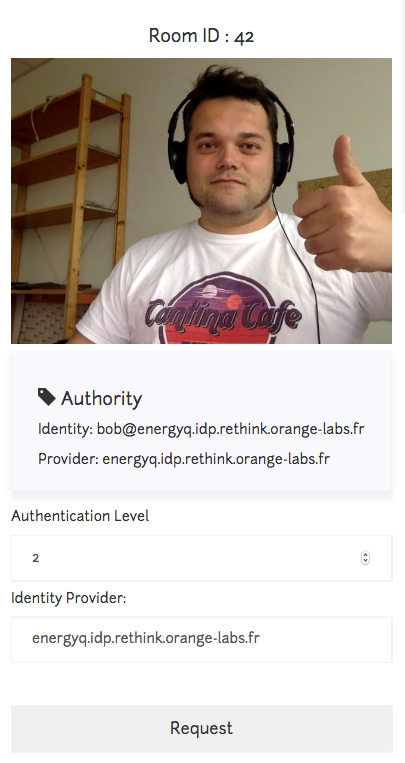
\includegraphics[width=\marginparwidth]{images/acor_negotiation}
\caption{Identity negotiation interface on a WebRTC service.\\\\}
\label{fig_acorNegotiation}
}

The \texttt{generateAssertion} function from the \gls{idp} Proxy has for parameters \texttt{contents}, \texttt{origin}, and \texttt{usernameHint}.
Request for a particular authentication class to the \gls{idp} is thus not defined.
We use the \texttt{usernameHint} parameters to pass \gls{acrus} parameters to the \gls{idp}.
The \gls{idp} is modified accordingly to understand this parameter.
However, the \texttt{IdentityValidationResult} dictionary do not represent the \gls{acrus}.
Dictionaries are JavaScript objects that cannot be extended by adding new members.
It is thus impossible for the validating \gls{idp} Proxy to return a certified \gls{acrus} value to the client inside the \texttt{IdentityValidationResult}.
In clear, even-though the client can request a particular authentication strength, it cannot verify that the \gls{idp} complied with the request.
A solution to solve this issue could be to let the client directly read the identity assertion contained by the \gls{sdp} message to check the asserted authentication strength.
The downside of such solution is that it loses the benefits of the WebRTC identity abstraction as the client must be able to natively understand the identity assertion.

It also appears impossible to change identity at call runtime or use multiples identities simultaneously.
The WebRTC specification states that if the PeerConnection object has \textit{"previously authenticated the identity of the peer [...], then this also establishes a target peer identity.
The target peer identity cannot be changed once set"}~\cite{w3c:webrtc}.
Our tests demonstrate that modifying the remote peer identity effectively closes the connection.
Once a first identity has been set, it cannot be changed.
If this is an issue and if several \gls{idp}s are available, the peer should first wait to receive an \gls{acor} attribute from the other peer, before setting an \gls{idp} for the session.

In the end and to answer RQ2.1, we are able to establish two anonymous sessions and then request the other peer to authenticate with a particular identity domain.
We are however unable to verify the strength of the authentication, hampering the capability to request a particular authentication strength.
In addition, our modified \gls{sdp} messages are effectively ignored by other services and by the user-agent.
Interoperability with other services should not be compromised by this new attribute.
Our observations are summarised in Table~\ref{tab:acor} which shows for both \gls{orus} and \gls{acrus} parameters whether they can be passed as input to the assertion generation function and returned as output of the assertion validation function.

\begin{table}
\begin{tabular}{@{}lcc@{}}\toprule\toprule
    Parameter & Can be set (input) & Can be verified (output)\\\midrule
  Origin Request & $\checkmark$ & Specified \\
  Authentication Class Request & $\checkmark$ & $\times$ \\\bottomrule
  \hline
\end{tabular}
\caption{Capability to Implement the Proposed Solution}
\label{tab:acor}
\end{table}

\section{WebConnect}
\label{webconnect}

In Section~\ref{sec:privacy}, we presented some privacy threat mitigation techniques, amongst which is data minimisation.
Authorization delegation frameworks give users some control over the information they want to share to other websites.
Used as \gls{sso} solutions, they put users in a situation where they have to choose between the burden of setting up a new account or sharing some private information.
%While \gls{idp} should offer privacy-friendly solutions, websites also have a responsibility as clients of these solutions.
Allowing users to choose privacy-preserving solutions may be an incentive for providers to respect their user's privacy.
However, we have shown in Section~\ref{userschooseidp:h1} that many websites abuse users' privacy by requesting unnecessary privacy-sensitive data.
In addition, Vapen et al.~\cite{DBLP:conf/sec/VapenCMS15} observed that in practice \gls{rp} offer few choices of \gls{idp}, an observation confirmed by our study (see Section~\ref{userschooseidp.study}).
We thus believe that users should be given more control over which \gls{idp} they want to use when authenticating on the Web.

In Section \ref{userschooseidp}, we consider some of the reasons that could prevent the implementation of \gls{idp} discovery mechanisms.
We estimate that at least 58\% of observed websites could make use of an \gls{idp} discovery mechanism.
However, we also found several hindrances to the deployment of such solution:
\begin{itemize}
\item the lack of implementation of this feature by \gls{idp} and \gls{rp}.
\item the difficulty for users of knowing and entering their identifiers in the discovery process.
\item the possible trust relations between the \gls{idp} and \gls{rp}.
\end{itemize}

Several tentatives have been made to develop Internet's ``Missing Identity Layer''~\cite{cameron2005laws}, without clear success.
A proposition of the ``Seven Laws of Identity''\cite{cameron2005laws} is that a single protocol would not fit all needs on the Web, but that ``different identity systems must exist in a metasystem''. 
This implies the need for a simple encapsulating protocol and a unified user experience.
First released in 2007, Windows CardSpace\cite{chappel2006cardpace} was an implementation of an Identity Metasystem~\cite{jones2005microsoft} and Microsoft's solution to propose an integrated identity management experience to Windows' users.
It allowed users to select InfoCards to prove identity claims, \eg name, age, to requesting applications, as presented in Figure~\ref{fig:cardspace}.

\begin{figure}
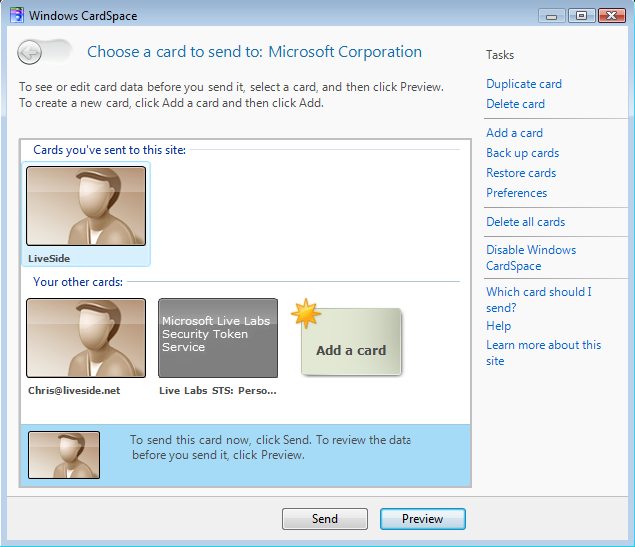
\includegraphics[scale=.5]{images/cardspace}
\caption[CardSpace User Interface]{CardSpace user interface. When a website requests an authentication, the CardSpace user interface prompts the user with a choice of identity cards. The user interface displays the identity of the requesting website and the user can select one identity card to present to the website. Alternatively, he can preview data contained by his cards, modify them, or add a new one. }
\label{fig:cardspace}
\end{figure}

An identity aware web browser would have several advantages.
In their 2011 empirical study, Sun et al.~\cite{Sun2011} observe users concerns about web \gls{sso} and recommend that ``identity support into the browser [would provide user with] a consistent, intuitive and trustworthy user experience''.
We also note that our survey presented in Section~\ref{sec:devsurvey} reveals that by default the authentication strength, the complexity of implementation, and the user experience are the most important factors for developers when considering to implement an \gls{sso} solution.
A web Identity Metasystem should thus aim to offer these advantages to developers in order to facilitate its adoption. 

Recent trends in web browser development tend to indicate that browser makers are looking to offer a complete browser experience.
Personal preference synchronisation, official plugins bringing new functionalities\footnote{Firefox Hello was a WebRTC service integrated with Firefox. It was released with the Firefox 35 update, but later discontinued since Firefox 49.}, or simply access to an application marketplace. 
Particularly related to our interest, Google Chrome offers an OAuth~2 \gls{api}\footnote{\url{https://developer.chrome.com/apps/app\_identity}} to Chrome Apps\footnote{Chrome Apps are third-party web applications running inside Chrome.}.
This \gls{api} implies that users can use a Chrome interface to choose an identity, sign-in, and modify some of their information such as their profile picture.
However, Chrome only offers integration with Google's identity.

The WebRTC identity specification also enriches the browser with a kind of identity management capability but limited to the scope of WebRTC user-to-user authentication.
As we described already, the specification offers interesting features.
Firstly, it offers an \gls{idp} discovery functionality by serving the \gls{idp} Proxy from \texttt{/.well-known} standard location on the \gls{idp}.
And secondly, the WebRTC identity specification exposes a simple protocol for authentication based on the generation, exchange, and verification of identity assertions.
We believe that an identity-enabled web browser exposing an authentication \gls{api} to websites could be the basis for a new web Identity Metasystem.
The browser would provide the functionalities and associated interfaces to configure new identities, register passwords, display login prompt, and define website preferences, \ie which identity to use with which web site.
Some of these functionalities are already provided by web browser, \eg login and password storage, but without the coherency of a full identity management experience. 

The \gls{idp} Proxy is the core component of the WebRTC identity architecture.
It is discoverable and exposes the \gls{api} for handling identity assertions.
Theoretically, it is also protocol independent and we proposed multiple implementations of this component in Section~\ref{idpproxyimplem}.
In this Section, we address RQ3 ``can we let users chose actors they trust to participate in the communication setup?''.
More precisely, we are interested in answering the following research question:
\begin{itemize}
    \item \textbf{RQ3.4}: Can we leverage the WebRTC identity architecture to let users chose their \gls{idp} for user-to-server authentication?
\end{itemize}

\subsection{Implementation}
To answer our research question, we implement a prototype of a browser modification\footnote{\url{https://github.com/Sparika/WebConnect}}.
Our proposed architecture (see Figure~\ref{fig:webconnectarch}) relies on three components interacting together: 
\begin{itemize} 
\item A JavaScript \gls{api} accessible to websites and a user interface for identity selection. Providing a web \gls{api} is necessary for WebConnect to be a standard functionality of web browser and facilitate its integration by developers.
\item An \gls{idp} Server able to provide a suitable identity assertion through a WebRTC compatible \gls{idp} Proxy. 
\item An \gls{rp} website \---client and server side\--- able to understand and verify the provided identity assertion
\end{itemize}

\begin{figure}
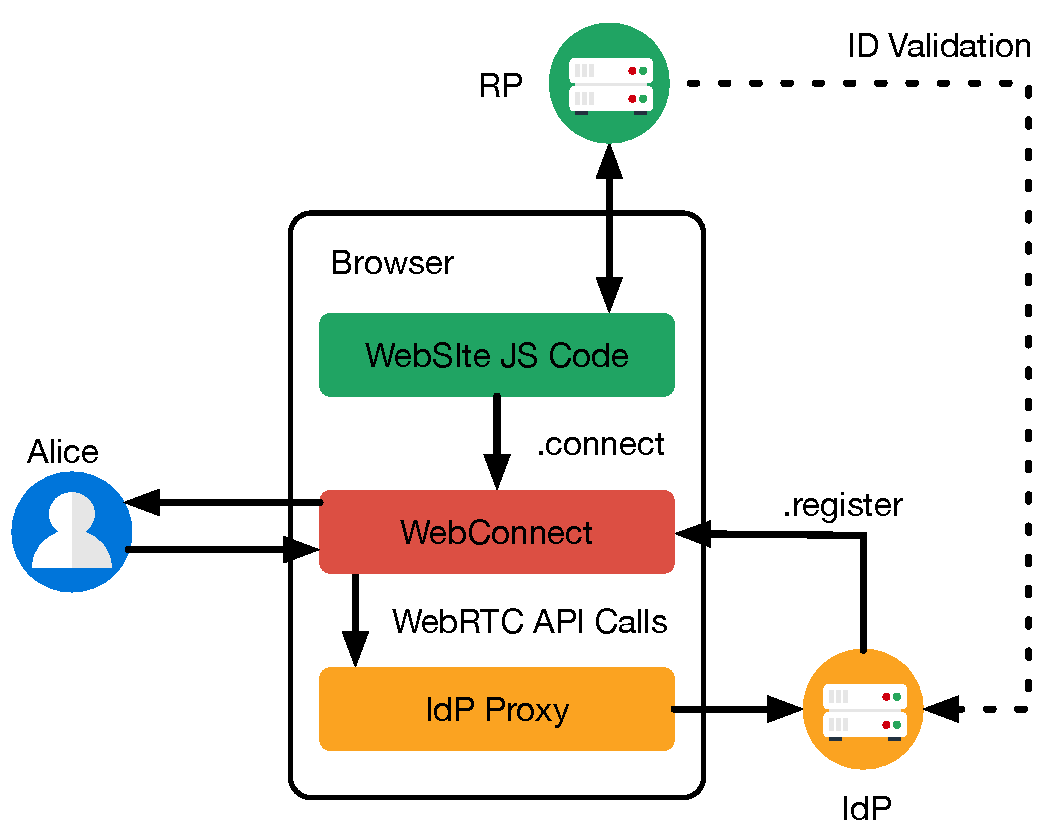
\includegraphics[scale=.5]{images/webConnect.pdf}
\caption{WebConnect Architecture}
\label{fig:webconnectarch}
\end{figure}

Figure~\ref{fig_seqapi1} shows sequence diagrams representing the interaction between the different actors of our implementation. 
After the user requested to login, the JavaScript client code calls the \texttt{WebConnect.connect} function which returns a promise for an identity assertion.
The browser then asks the user to choose one of its registered identity providers and then proceed to instantiate the corresponding \gls{idp} proxy. 
%Interactions with the instantiated \gls{idp} proxy follows the WebRTC identity specification.
Once the \gls{idp} Proxy returns the identity assertion to the browser, the browser resolves the \texttt{connect} promise and the website client receives the assertion.
It is then up to the client code to transfer the assertion to the server side.
In our example, the client calls the GET method on a login \gls{url} and passes the assertion as a \gls{url} query parameter. 
The server then extracts the \gls{jku} parameter from the identity assertion header, and get the public key from the \gls{idp} over \gls{https} at the provided location.
This public key is then used to verify the assertion signature.
%The format and verification procedure of the assertion are detailed in Section~\ref{sec_assert}.
Once the assertion authenticity and integrity is confirmed, the server logs in the user and responds to the client GET.

\begin{figure*}[tbp]
\begin{center}
        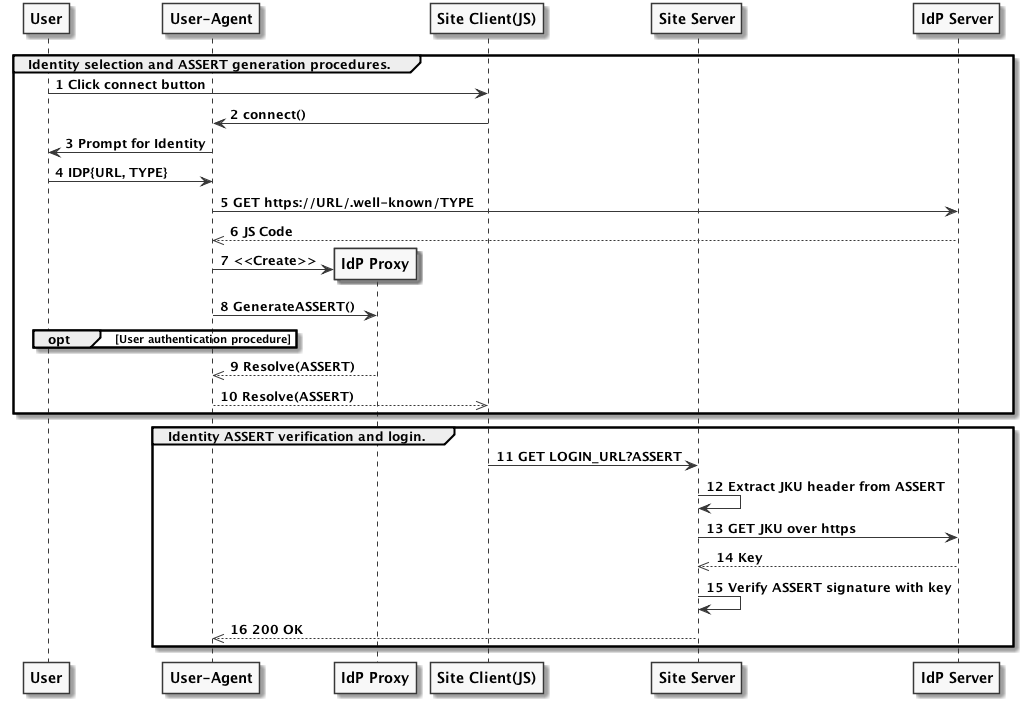
\includegraphics[height=\textwidth, angle=90]{images/connectAPI}
\end{center}
        \caption{WebConnect identity assertion management sequence diagram.}
        \label{fig_seqapi1}
        \label{fig_seqapi2}
\end{figure*}

\subsubsection{Browser modification}
Our browser modification takes the form of a browser extension.
This solution was chosen for its simplicity in comparison to browser source modifications. 
As a browser extension does not expose function to the global window scope, its exposed functions cannot be called by a website.
To simulate access to a web \gls{api}, we also provide a JS shim exposing our \gls{api} functions to the website client code.
This script can then communicate with the extension code through the \texttt{postMessage} \gls{api}.

The \gls{api} exposed by the \texttt{WebConnect} object offers two functions: \texttt{connect} and \texttt{register} as specified in Figure~\ref{WebConnectWebIDL}. 
The register function is called by the \gls{idp} to let users store identity cards in the browser.
The \texttt{iss} and \texttt{type} parameters allows to discover the \gls{idp} proxy \texttt{/.well-known} location, while \texttt{sub} is an identifier for the user on the \gls{idp}.
\texttt{name} and \texttt{picture} are used for display on the user identity card.
The \texttt{connect} function is called by websites to request an identity assertion authenticating the user. 
Its only parameter is a \gls{json} object to convey additional parameters such as constraints, authentication level, or authorization requests.
We do not implement scenario using this parameter, although we discuss possible usages in Section~\ref{extensions}.

\begin{figure}[H]
\begin{Verbatim}[commandchars=\\\{\}]
interface \textcolor{matred}{WebConnect} \{
    \textcolor{matblue}{void} register (\textcolor{matred}{String} iss,
           \textcolor{matred}{String} proxy,
           \textcolor{matred}{String} sub,
           \textcolor{matred}{String} name,
           \textcolor{matred}{String} picture);
           
    \textcolor{matblue}{Promise<JWT>} connect(\textcolor{matred}{Object} request);
\};
\end{Verbatim}
\caption{WebConnect interface specification in WebIDL.}
\label{WebConnectWebIDL}
\end{figure}

On the technical side, our extension implements a graphical user interface for identity selection and configuration on top of the \texttt{PeerConnectionIdP} Firefox module. 
As we leverage and reuse the WebRTC identity specification, we developed our prototype for Firefox which is the only browser to support it.
Initially the extension was using the Firefox Add-on \gls{sdk} and in particular the \texttt{chrome} module.
This module allows accessing privileged low-level \gls{api}.
We were thus able to load the \texttt{PeerConnectionIdP.jsm} module and directly instantiate and interact with the \gls{idp} proxy through it.
However, the Firefox Add-on \gls{sdk} is being deprecated in favor of the WebExtension \gls{api}\footnote{The WebExtension \gls{api} is compatible with the Browser Extensions \gls{api}, a cross-browser effort supported by a \gls{w3c} Community Group for interoperable extensions~\cite{w3c:browserext}.}.
Extensions developed with these \gls{api} cannot use browser specific low-level \gls{api} such as the \texttt{chrome} module.
In order to instantiate the \gls{idp} proxy and get the identity assertion, the extension now instantiates a new \texttt{RTCPeerConnection}.
Though the connection is never initiated, the \texttt{RTCPeerConnection} object can be used to call the \texttt{setIdentityProvider} and \texttt{getIdentityAssertion} functions.
While this effectively allows the extension to retrieve an identity assertion, the  \texttt{RTCPeerConnection.getIdentityAssertion} functions offers less control than the one exposed by the \texttt{PeerConnectionIdP.jsm} module. 

\subsubsection{Identity provider implementation}
\label{sec_assert}
The role of the \gls{idp} is to provide an \gls{idp} Proxy at a standard location, and through it, authenticate the user and return an identity assertion.
We reuse our \gls{oidc} \gls{idp} Proxy implementations described in Chapter~\ref{webrtcprivacy}.
The returned assertion is thus a signed \gls{jwt}.
In WebRTC the party wanting to verify the assertion validity is supposed to also download the \gls{idp} proxy to verify the assertion. 
However, as we wanted to avoid \gls{idp} Proxy sandboxing on the website server, we used the \texttt{jku} header in the \gls{jwt} assertion. 
This allows the verifying party to retrieves, from the \gls{idp}, the public key used to sign the assertion and verify the \gls{jwt} authenticity.
%\todo{Pour une raison de s�curit� je me suis dit que l'ex�cution c�t� serveur du proxy �tait � �viter. Mais avec le recul, si on autorise le sandboxing c�t� client, pourquoi ne pas l'autoriser c�t� serveur. Du coup est-ce qu'il y aurait d'autres raisons qui pourrait justifier a posteriori? Par exemple niveau performances. http://gf3.github.io/sandbox/}
%\todo{Simon:Mais  le client est un TEE, c'est une des hypoth�ses. Qu'en est-il du serveur?}

As standard for \gls{oidc}, the assertion payload contains Issuer Identifier (\texttt{iss}) and Subject Identifier (\texttt{sub}), respectively identifying the \gls{idp} and the user to the requesting website. 
The payload may also include \gls{oidc} user-info claims, such as name, address, or email.

\subsubsection{Website implementation}
Besides calling the \gls{api} to get an identity assertion, a compatible website must also be able to understand and verify the assertion.
In our prototype implementation, the JavaScript code on the client side sends the assertion to its backend server for verification and log in. 
This is done by a GET to a login \gls{url} with the assertion transmitted as a URL query parameter. 

The assertion authenticity is then verified by the server. 
To do so, developer can use several libraries for \gls{jwt} support.
We implement a \gls{jwt} strategy for Passport\footnote{http://passportjs.org/} \---a popular NodeJS authentication library\--- by adding support for \gls{jku} verification.
Once the assertion has been verified, the server extracts relevant information from it and lookup for existing users in its database.
If no user exists, the server creates a new entry on the fly. 
The login procedure thus serves the dual purpose of enrolment and authentication.
Ultimately, the user is returned to the relevant page through the \gls{http} response. 

\subsection{Analysis}
\subsubsection{Security analysis}
In comparison to a standard OAuth~2 flow, our implementation introduces two major changes that may have security implications.
We discuss these changes in this section.

Firstly, in order to verify the validity of claims covered by a received assertion, the \gls{rp} must verify the assertion's signature.
In OAuth~2 this signature would have been produced by the \gls{idp} using a key pair exchanged with the \gls{rp} during the registration process.
In our solution, we replaced the registration process, including the key exchange, by a verification of the \texttt{jku}'s  origin.
However, the OpenID Connect specification states "ID Tokens SHOULD NOT use the JWS [...] jku, or jwk header parameter fields".
From \gls{ietf} mail archives\footnote{\url{https://www.ietf.org/mail-archive/web/jose/current/msg03929.html}}, it appears that assertions claims, including the \texttt{iss} and \texttt{jku} parameters, are considered to be self asserted until verified by a trusted key. 
To solve this issue, additional constraint could be added to the key's origin verification.
For instance, using a standard \texttt{/.well-known}~\cite{RFC5785} path for the \texttt{jku} \gls{url} also matching the \texttt{iss} domain would prevent attacker from specifying any key.
We note that similarly, the WebRTC identity specification specifies that the identity's origin and \gls{idp} proxy's origin must match and be served with the \gls{https} protocol.
Imposing the same constraint for \gls{jwt} verification should provide a similar security level.

Secondly, assertions manipulated by the javascript client code and returned by the \gls{api}'s promise response are added to the page's global scope.
The assertion could thus be read, and used, by a malicious cross-origin script embedded on the same page.
This issue is similar to what can happen on an OAuth~2 implicit flow, where the client directly receives an access token.
In OAuth~2, the code flow lets the client exchange a code and authentication with the token endpoint to get the access token, and the ID token in \gls{oidc}.
But as in our solution, the \gls{rp}/client cannot be authenticated by the \gls{idp}, the code flow cannot be used.
An alternative solution could be to use a sort of code exchange, leveraging \gls{tls} mutual authentication between the \gls{rp} and \gls{idp}.
Alternatively, the browser could protect the assertion from the JavaScript code and transmit it directly to the \gls{rp} sever.
Action 10 and 1 from Figure~\ref{fig_seqapi1} would be replaced by a single message from the User-Agent to the Site Server.
The website redirection \gls{uri} would be passed as a parameter to the connect function during action 2 on Figure~\ref{fig_seqapi1}.


\begin{figure}
\centering
\begin{subfigure}{\textwidth}
        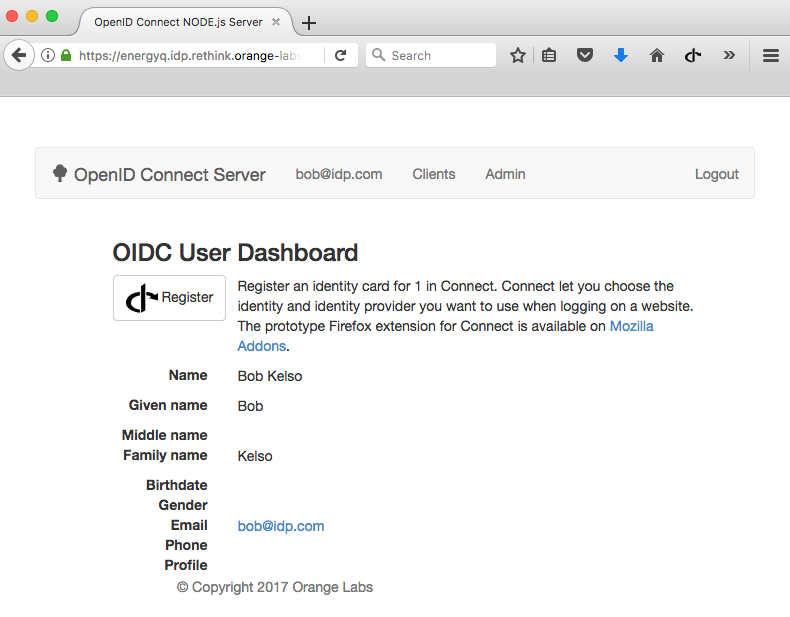
\includegraphics[width=\textwidth]{images/acor_login7}
        \label{fig:prototype:3}   
        \caption{IdP profile page with the WebConnect register button.}
\end{subfigure}    
\begin{subfigure}{\textwidth}
        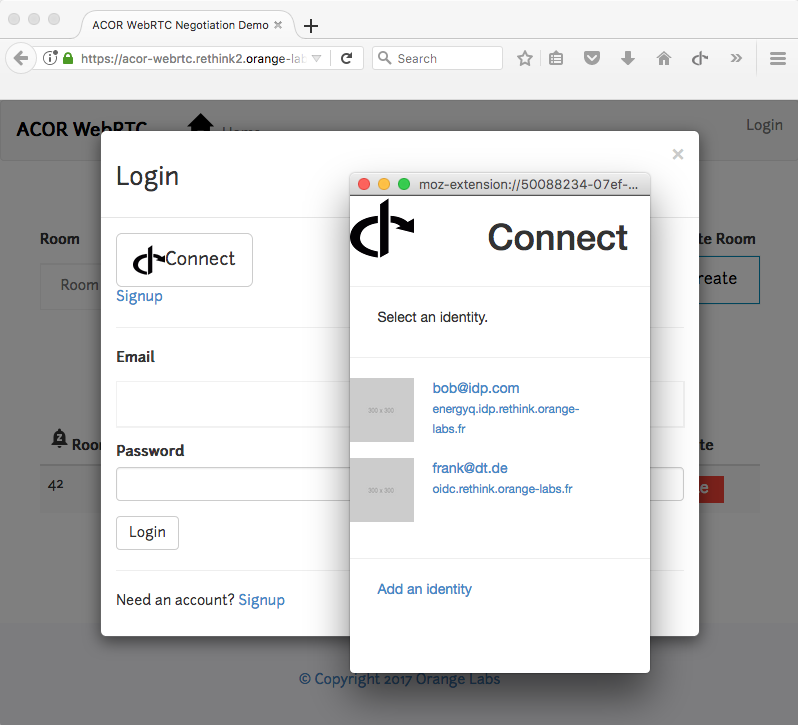
\includegraphics[width=\textwidth]{images/acor_login0}
        \label{fig:prototype:1}   
        \caption{Web Connect identity selection interface}
\end{subfigure}
%\begin{subfigure}{\textwidth}
%        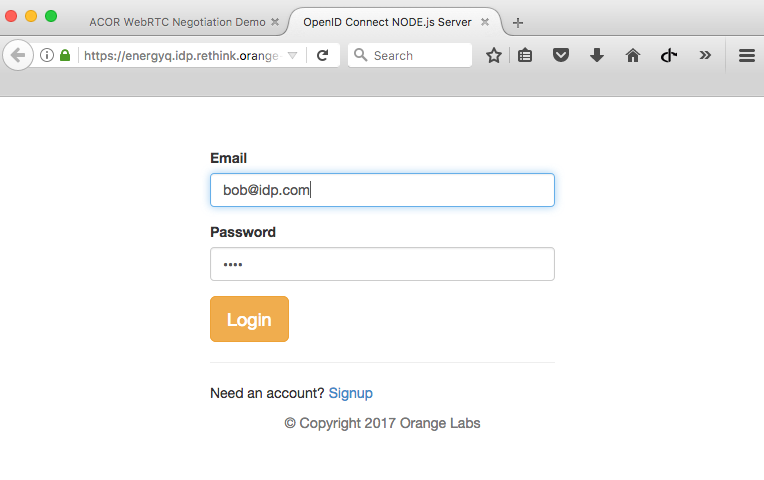
\includegraphics[width=0.5\textwidth]{images/acor_login4}
%        \label{fig:prototype:2}   
%        \caption{Hello}
%\end{subfigure}        
%\begin{subfigure}[b]{0.5\textwidth}
%        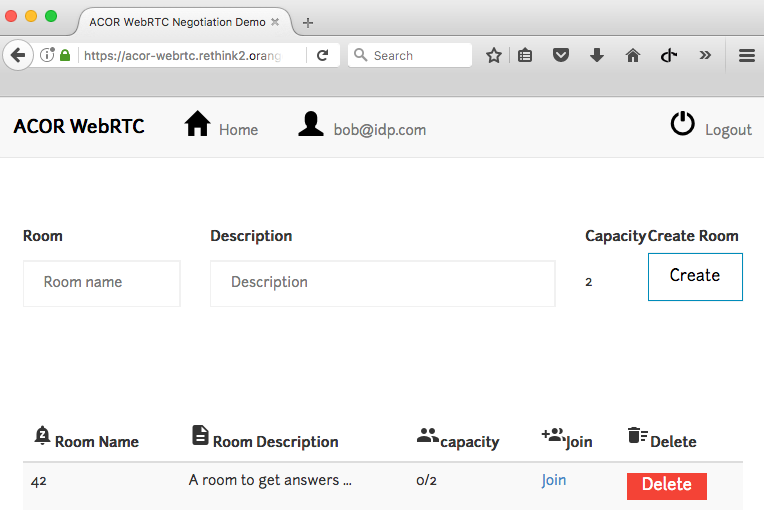
\includegraphics[width=\textwidth]{images/acor_login5}
%\end{subfigure}         
        \caption[Prototype user interface for the Authentication web \gls{api}.]{Prototype user interface for the Authentication web \gls{api}.\\\\
        (a): The IdP profile page allows the user to configure a new identity cards to WebConnect. Clicking on register calls the \texttt{WebConnect.register} function.\\\\
        (b): On the visited website, the user can click on connect to authenticate. 
        This opens the WebConnect user interface and allows the user to choose the identity the user wants to authenticate with.}
        \label{fig_prototype}   
\end{figure}

\subsubsection{Usability}
From the end-user perspective, the overhead is quite limited. 
Compared to current authentication process, users have to register their identity cards on their browsers. 
This configuration can be done in a single action with the \texttt{register} function of the \gls{api}. 
Identity selection on login request is also similar to current \gls{sso} solutions, for instance comparing to Google's identity selection interface in Figure~\ref{fig:googleIdSelector}. 
If that is an issue, preferences storage by the browser may help reduce it further. 
However, the user experience does not constitute our field of expertise and we did not conduct user studies.

On the developer side of things, we also evaluate the additional work to be limited.
Table~\ref{tab_dev} compares the number of new code lines for our prototype implementation compared to the total code lines of each module.
In proportion, the biggest tasks are to develop the browser modification and the \gls{idp} Proxy, which are new concepts. 
We note that these developments would be done once by browser makers and \gls{idp} developers and not by web developers.
For client website developers, the main task is to configure the new authentication method and verify the assertion authenticity.
However, as we noted, library for \gls{jws} and \gls{oidc} ID Token support already exists.
Modifying the existing \gls{jws} verification library required 60 new lines over a total 1242 code lines, while configuring the new strategy required 70 code lines, mostly copy-pasted from other strategies.

\begin{table}
\centering
\begin{tabular}{@{}lcc@{}}\toprule\toprule
  Module & Total code lines & New code lines\\\midrule
  Firefox Addon & 0 & 417\\
  IdP Proxy & 0 & 197\\
  Client site (.js) & 693 & 66\\
  Client site (.conf) & 457 & 70\\
  Passport JWS & 1242 & 60\\\midrule
  Total & 2392 &  810 \\\bottomrule
  \hline
\end{tabular}

\caption{Code lines written for the prototype implementation}
\label{tab_dev}
\end{table}

The objective of an Identity Metasystem is to offer a simple \gls{api} to access multiple identity services.
On the long run, the adoption of a web \gls{api} for authentication delegation should reduce the amount of work for web developers.

\subsection{Validation}
\label{extensions}
We present a prototype of a user-to-server authentication mechanism reusing already implemented \gls{idp} Proxy.
Integrated into an identity selector interface provided by the web browser, it effectively allows users to select trusted \gls{idp} for authentication on compatible websites.
Due to the identity continuity principle (see Section~\ref{sec:webrtcidpath}), such freedom of choice would extend to user-to-user authentication in WebRTC context.
Through experiment, we answer RQ3.4 and demonstrate that the WebRTC identity architecture can be leveraged to build a user-to-server authentication mechanism.
We thus believe that a web Identity Metasystem such as WebConnect is a good way to give users more control over which identity services they want to use both in WebRTC and on the Web in general.

Nonetheless, some control may have to remain in the hands of \gls{rp} websites.
In Section~\ref{userschooseidp} we classified at least 58\% of observed \gls{rp} websites as authentication or profile. 
Websites from this class could request user's authentication without any scope or authorization constraints.
We also observed that some \gls{rp} websites may have a trust relationship with some \gls{idp}.
Our conclusion stated that ``a solution to simplify the discovery and registration of \gls{idp} endpoint should nonetheless give \gls{rp} the option to control the range of compatible \gls{idp} and the authentication strength''.

The \texttt{request} parameter of the \texttt{WebConnect.connect()} function allows \gls{rp} websites to specify constraints on the range of compatible \gls{idp} when calling the \gls{api}.
This parameter thus serves as a hook for future extensions allowing to specify: 
\begin{itemize}
\item trusted \gls{idp}'s origin,
\item authentication strength requests,
\item and required scopes for authorization.
\end{itemize}
These constraints would then be used by the WebConnect interface to only display to the user a range of compatible \gls{idp}.
%Additionally, the \texttt{request} parameter can be used as a way to specify parameter for the \gls{idp} Proxy and the \gls{idp}.
Note that the \gls{idp}'s origin and authentication strength constraints are similar to how we described users negotiating authentication of the other peers in Section~\ref{sec_sdp}.

%\clearpage
\invisiblesection{Summary}
\label{sec:c2Summary}
\vspace*{3cm}

\blockmargin%
\hspace{-\marginparwidth}\hspace{-\marginparsep}
\makebox[\overflowingheadlen][l]{
\begin{minipage}{\overflowingheadlen}

\begin{mdframed}[style=C2Frame,frametitle={\ref{sec:c2Summary}~Summary}]

In some WebRTC scenarios, users may not trust their communication service or the signalling layer.
Using the WebRTC identity architecture, users instead rely on \gls{idp} to bind the signalling to a peer-to-peer authentication.
In such case, users trust in these \gls{idp} and their authentication process is necessary for the communication to be trusted.
In this chapter, we have looked at solutions to give users more control over WebRTC identity parameters: their peer authentication and their own \gls{idp}.

\medskip

Firstly, we presented \gls{acor}, a \gls{sdp} extension to negotiate the Authentication Class and the \gls{idp}'s Origin for the authentication of the other party during a WebRTC call.
We implemented our solution in a WebRTC service and tested it using Firefox to answer RQ2.1.
Our tests reveal that while it is possible to request identity parameters to the other peer, obtaining feedback on the peer's authentication class is not possible at the moment.
We believe that this missing feature may be useful even outside of a negotiation use case and that it could easily be supported by the WebRTC identity architecture.

\medskip

We then presented WebConnect, a web identity metasystem to let users select their trust \gls{idp}.
WebConnect answers RQ3.4 and shows that the WebRTC identity architecture can be leveraged to build a user-to-server authentication mechanism.
We implemented a prototype version based on a Firefox extension and reusing \gls{idp} Proxy implemented in Section~\ref{idpproxyimplem}.
We believe that a web Identity Metasystem such as WebConnect is a good way to give users more control over which identity services they want to use both in WebRTC and on the Web in general.

\end{mdframed}

\end{minipage}
}
\unblockmargin